% !TeX root = ../main.tex

\chapter{系统测试}

系统测试的目的是将系统的功能实现与需求设计进行比较,发现系统中存在
的不满足用户需求的情况或者程序中存在的问题,从而对系统功能进行改进,
提高软件的可靠性。本章主要针对系统的功能性测试和非功能性测试进行介绍\cite{32}。

\section{系统功能性测试}

功能性测试使用的是Swagger,Swagger是一种RESTful API文档生成工具,
它可以帮助开发者更方便地描述、调用和测试API。使用Swagger可以自动生成API文档,
并提供一个交互式的UI界面,方便开发者查看和测试API接口。除此之外,Swagger还提供了许多有用的功能,
例如自动生成客户端SDK、自动生成API测试代码、集成Mock数据等。

\subsection{数据源管理}

在数据源页面,可以看到所有已创建的数据源,然后还可以对数据源进行创建、查看、编辑、删除功能,
支持的数据源有关系型数据库Mysql,消息队列数据源Tube、Kafka、Pulsar等数据源。
数据源的相关页面如图\ref{fig:创建数据源页面}所示。

\begin{figure}[H]
  \centering
  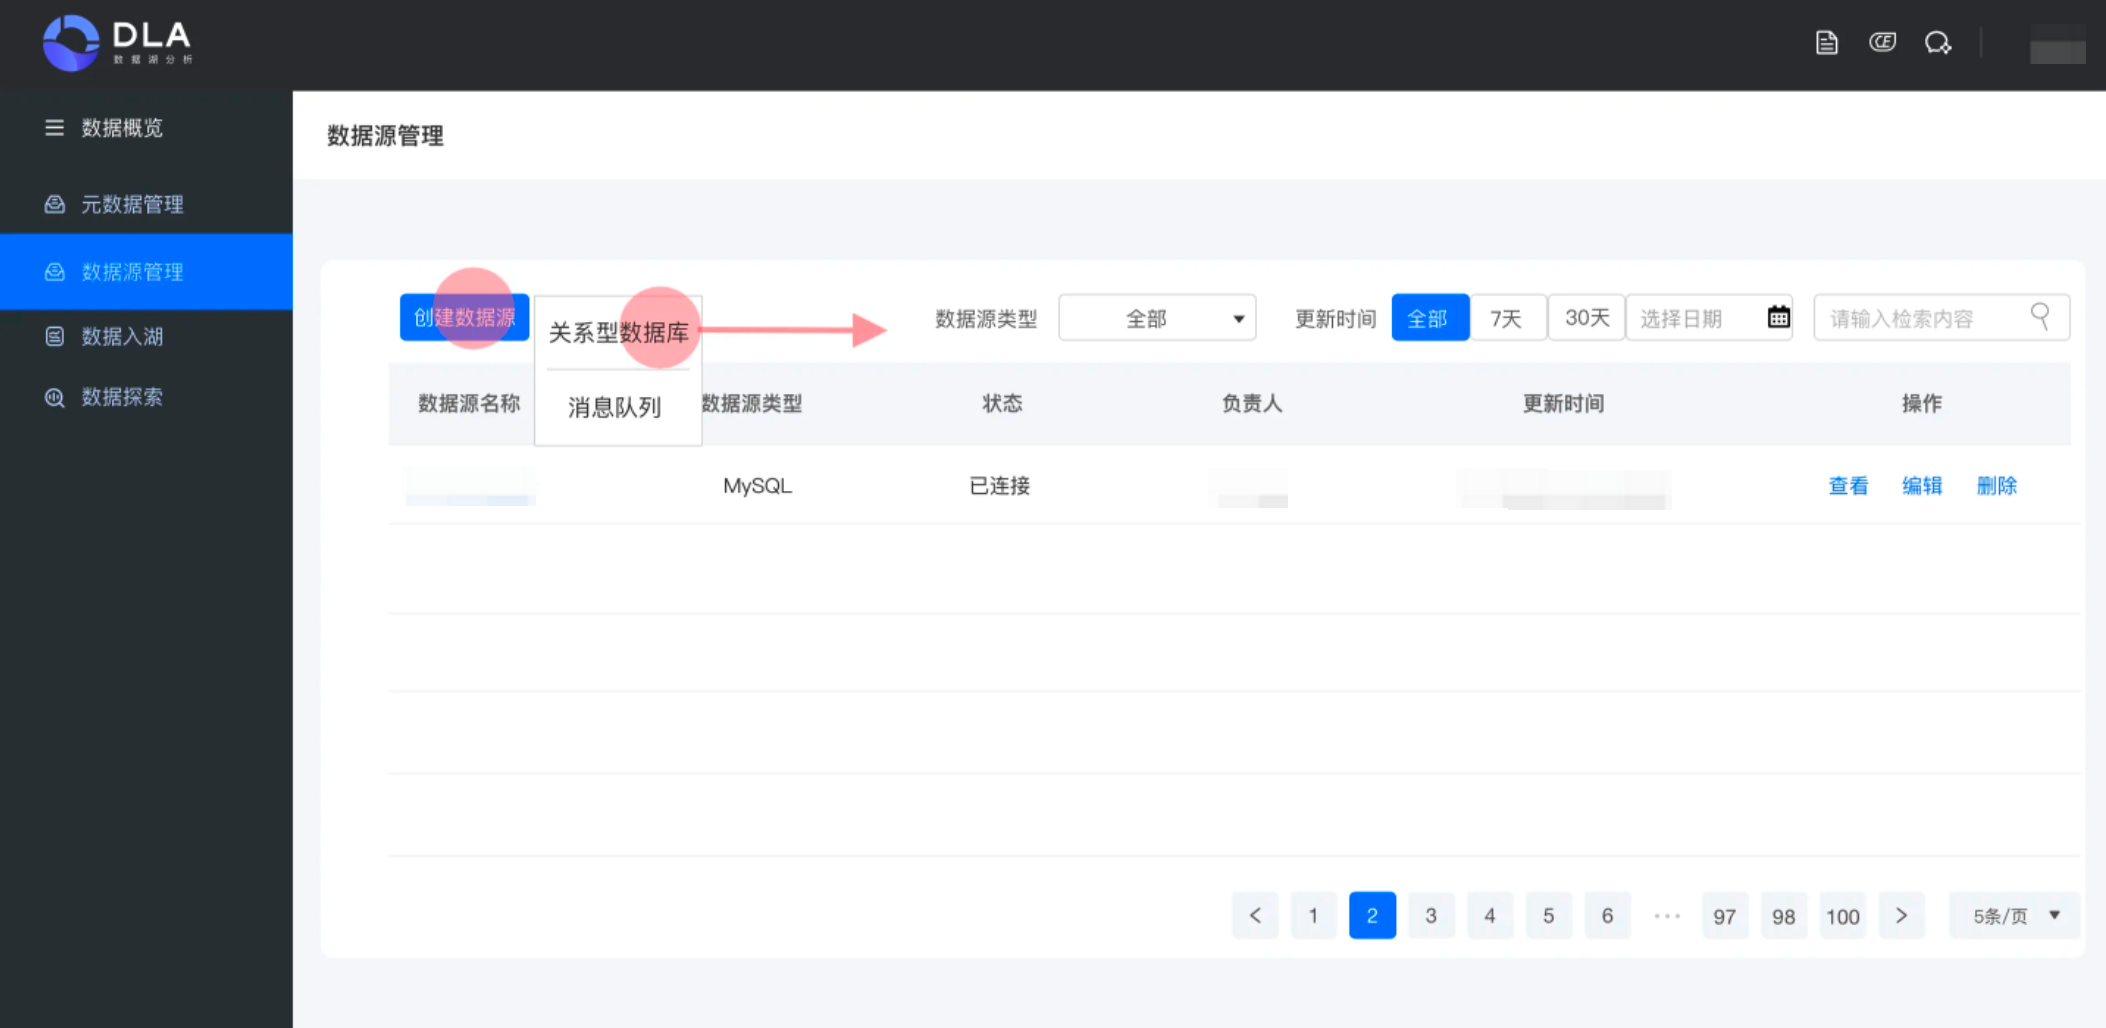
\includegraphics[width=1.0\textwidth]{创建数据源.png}
  \caption{创建数据源页面}
  \label{fig:创建数据源页面}
\end{figure}

这里仅展示创建MySQL数据源、获取数据源列表、测试数据源连通性的接口测试。

(1)创建Mysql数据源的接口测试如表\ref{tab:exampletable1}所示:

\begin{table}[H]
  \centering
  \caption{创建Mysql数据源接口测试}
  \label{tab:exampletable1}
  \begin{tabular}{ll}
    \toprule
    接口描述         & 创建Mysql数据源          \\
    \midrule
    测试类型         & 功能测试         \\
    前置条件         & 后端服务器、MySQL服务器正常         \\
    接口地址       & /formation/v1/datasource/createKafkaDatasource         \\
    请求方式         & POST      \\
    请求数据类型         & application/json     \\
    响应数据类型         & application/json,*/*           \\
    实际结果         & 达到预期结果           \\
    结论            & 测试通过           \\
    \bottomrule
  \end{tabular}
\end{table}

(2)获取数据源列表的接口测试如表\ref{tab:exampletable2}所示:

\begin{table}[H]
  \centering
  \caption{获取数据源列表接口测试}
  \label{tab:exampletable2}
  \begin{tabular}{ll}
    \toprule
    接口描述         & 获取数据源列表         \\
    \midrule
    测试类型         & 功能测试         \\
    前置条件         & 后端服务器、MySQL服务器正常         \\
    接口地址       & /formation/v1/datasource/getDatasourceList         \\
    请求方式         & GET      \\
    请求数据类型         & application/json     \\
    响应数据类型         & application/json,*/*           \\
    实际结果         & 达到预期结果           \\
    结论            & 测试通过           \\
    \bottomrule
  \end{tabular}
\end{table}

(3)测试数据源连通性的接口测试如表\ref{tab:exampletable3}所示:

\begin{table}[H]
  \centering
  \caption{测试数据源连通性接口测试}
  \label{tab:exampletable3}
  \begin{tabular}{ll}
    \toprule
    接口描述         & 测试数据源连通性         \\
    \midrule
    测试类型         & 功能测试         \\
    前置条件         & 后端服务器、MySQL服务器正常         \\
    接口地址       & /formation/v1/datasource/testConnectivity         \\
    请求方式         & POST      \\
    请求数据类型         & application/json     \\
    响应数据类型         & application/json,*/*           \\
    实际结果         & 达到预期结果           \\
    结论            & 测试通过           \\
    \bottomrule
  \end{tabular}
\end{table}

\subsection{元数据管理}

元数据是用于管理Iceberg表元数据的。在元数据管理页面,用户可以查看已创建的库和表,
以及关联自己在别处创建的Iceberg表元数据。通过元数据管理页面,用户还可以方便地查看和编辑
已创建的Iceberg表。对于编辑操作,元数据管理页面支持增加列、删除列、修改列的类型等多种操作,
这些操作都可以直接影响到表的结构和内容。除此之外,元数据管理页面还支持在数据优化方面的参数配置,
例如小文件合并、孤儿文件删除、过期快照删除、生命周期管理等,
这些参数的配置可以大大提高数据的查询和分析效率,同时也可以减少数据的存储空间和网络传输成本。
元数据管理的相关页面如图\ref{fig:元数据管理}所示。

\begin{figure}[H]
  \centering
  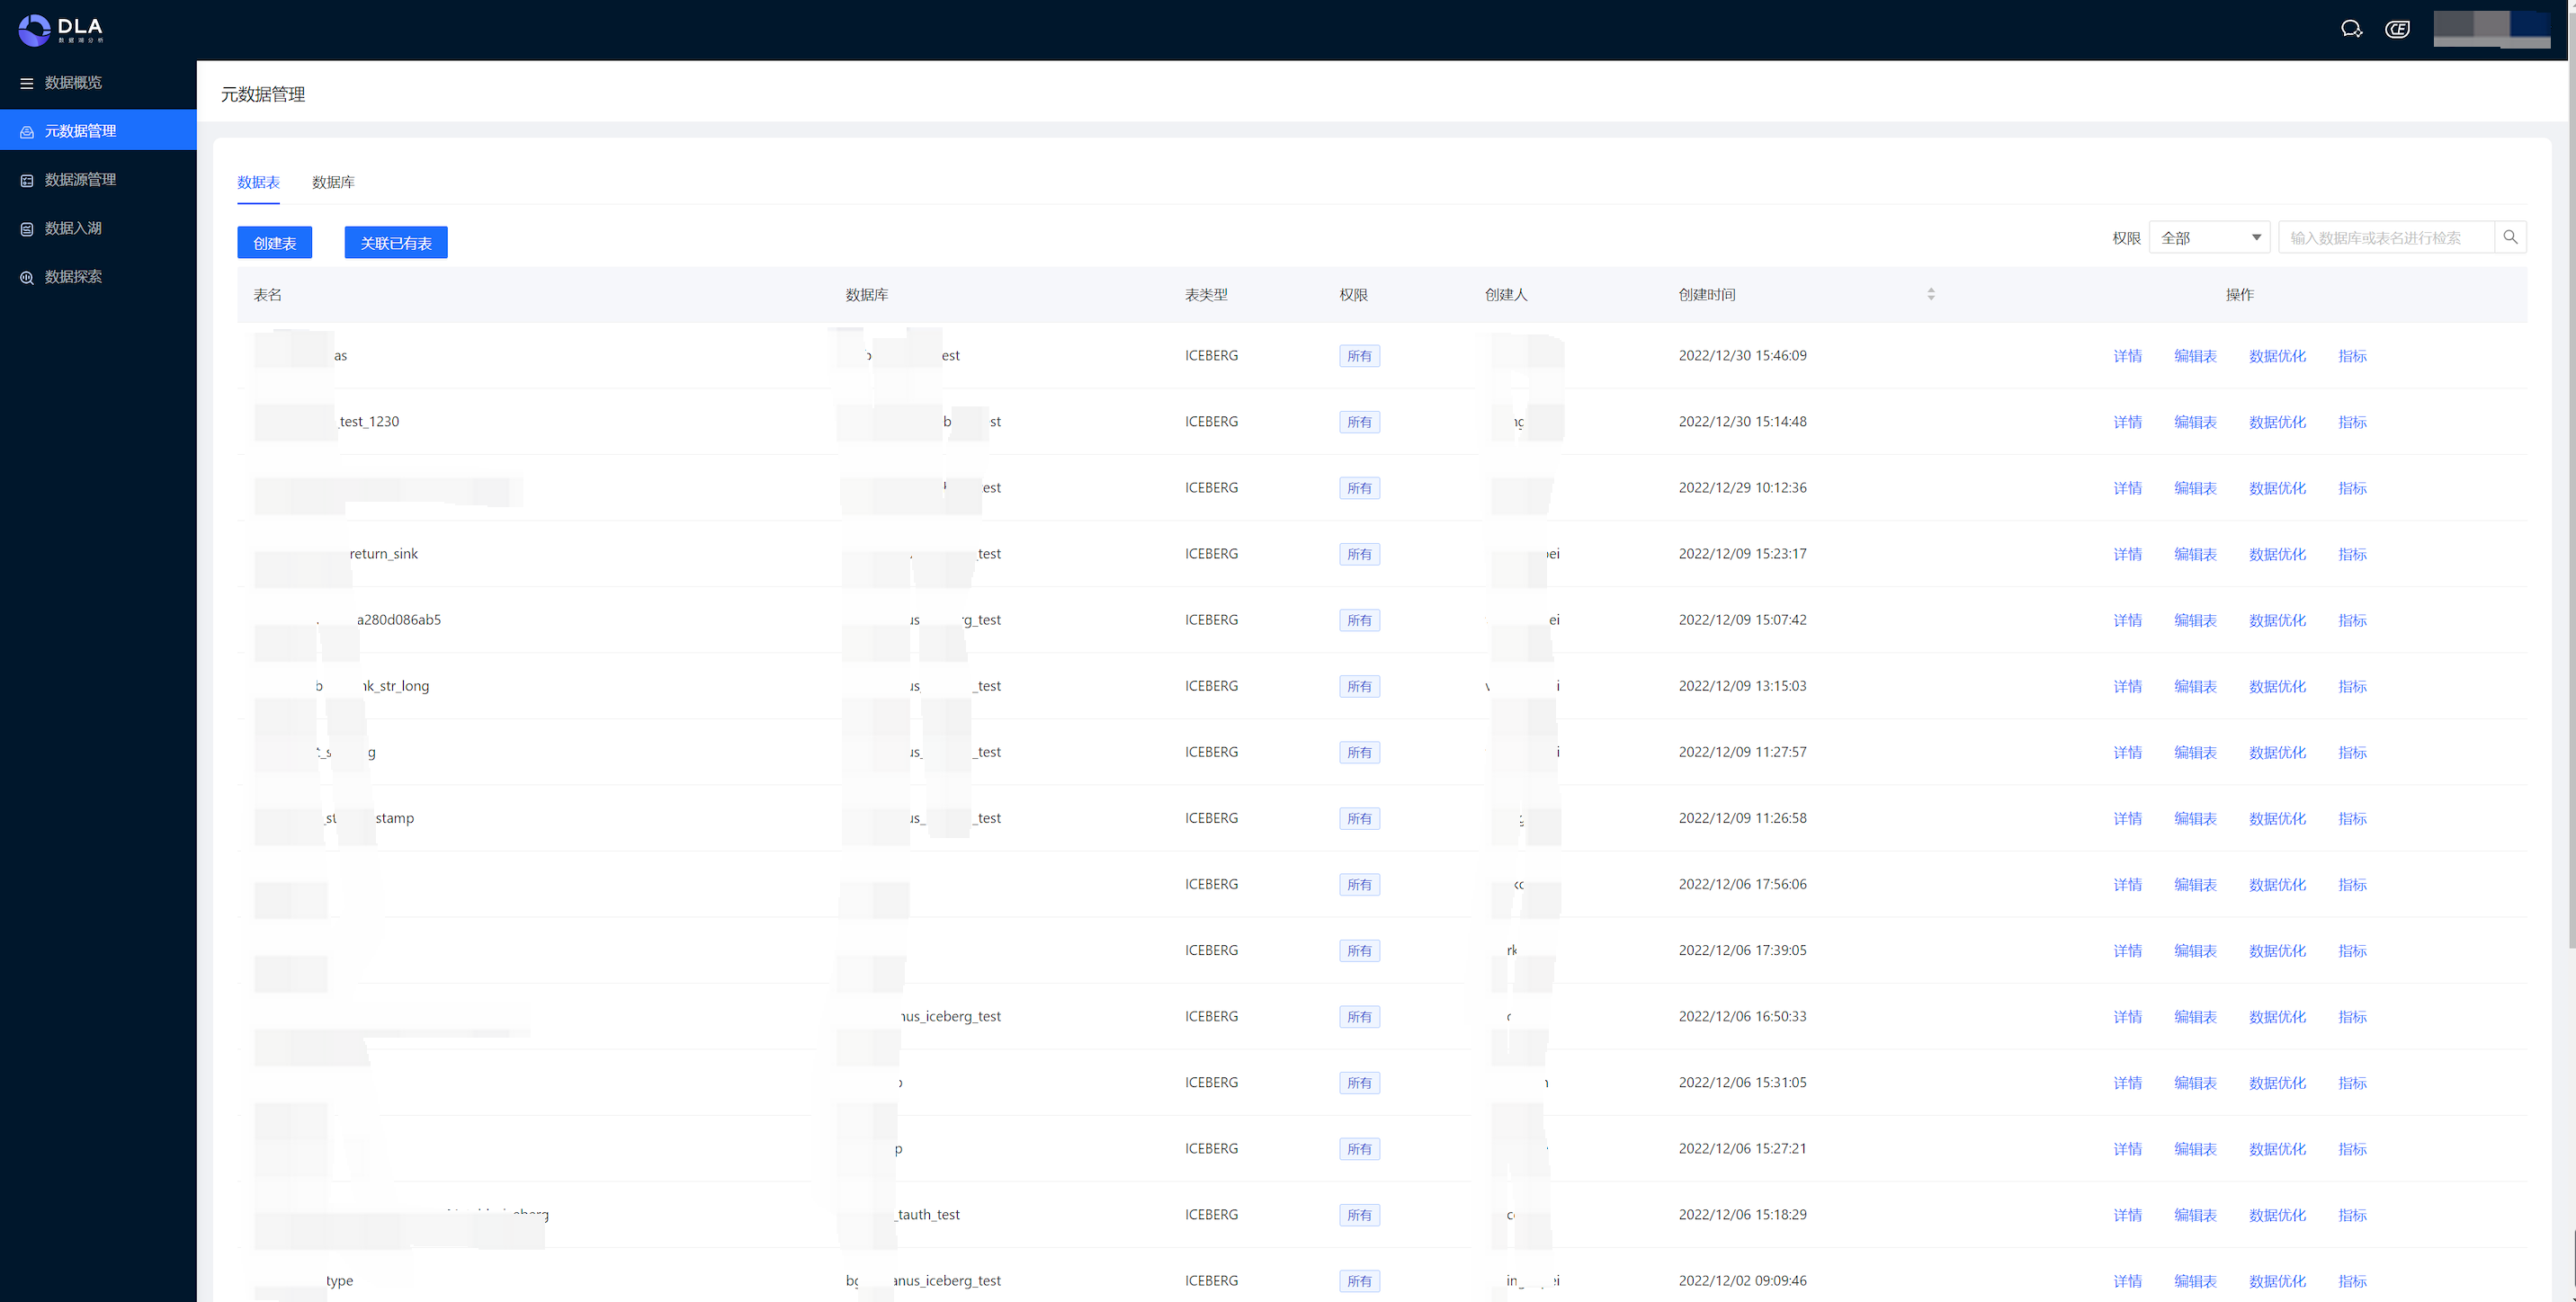
\includegraphics[width=1.0\textwidth]{元数据管理.png}
  \caption{元数据管理页面}
  \label{fig:元数据管理}
\end{figure}

相关的的接口测试如下:

(1)创建Iceberg表的接口测试如表\ref{tab:exampletable4}所示:

\begin{table}[H]
  \centering
  \caption{创建Iceberg表接口测试}
  \label{tab:exampletable4}
  \begin{tabular}{ll}
    \toprule
    接口描述         & 创建Iceberg表         \\
    \midrule
    测试类型         & 功能测试         \\
    前置条件         & 后端服务器、MySQL服务器、Hive Metastore服务正常         \\
    接口地址       & /formation/v1/metadata/createTable        \\
    请求方式         & POST      \\
    请求数据类型         & application/json     \\
    响应数据类型         & application/json,*/*           \\
    实际结果         & 达到预期结果           \\
    结论            & 测试通过           \\
    \bottomrule
  \end{tabular}
\end{table}

(2)关联已有表的接口测试如表\ref{tab:exampletable5}所示:

\begin{table}[H]
  \centering
  \caption{关联已有表接口测试}
  \label{tab:exampletable5}
  \begin{tabular}{ll}
    \toprule
    接口描述         & 关联已有表         \\
    \midrule
    测试类型         & 功能测试         \\
    前置条件         & 后端服务器、MySQL服务器、Hive Metastore服务正常         \\
    接口地址       & /formation/v1/metadata/associateTable        \\
    请求方式         & POST      \\
    请求数据类型         & application/json     \\
    响应数据类型         & application/json,*/*           \\
    实际结果         & 达到预期结果           \\
    结论            & 测试通过           \\
    \bottomrule
  \end{tabular}
\end{table}

(3)注册数据库接口测试如表\ref{tab:exampletable6}所示:

\begin{table}[H]
  \centering
  \caption{注册数据库接口测试}
  \label{tab:exampletable6}
  \begin{tabular}{ll}
    \toprule
    接口描述         & 注册数据库到数据湖         \\
    \midrule
    测试类型         & 功能测试         \\
    前置条件         & 后端服务器、MySQL服务器、Hive Metastore服务正常         \\
    接口地址       & /formation/v1/metadata/registerDatabase        \\
    请求方式         & POST      \\
    请求数据类型         & application/json     \\
    响应数据类型         & application/json,*/*           \\
    实际结果         & 达到预期结果           \\
    结论            & 测试通过           \\
    \bottomrule
  \end{tabular}
\end{table}

(4)获取表列表测试用例如表\ref{tab:exampletable7}所示:

\begin{table}[H]
  \centering
  \caption{获取表列表接口测试}
  \label{tab:exampletable7}
  \begin{tabular}{ll}
    \toprule
    接口描述         & 获取指定库下的表         \\
    \midrule
    测试类型         & 功能测试         \\
    前置条件         & 后端服务器、MySQL服务器、Hive Metastore服务正常         \\
    接口地址       & /formation/v1/metadata/getTableList        \\
    请求方式         & GET      \\
    请求数据类型         & application/json     \\
    响应数据类型         & application/json,*/*           \\
    实际结果         & 达到预期结果           \\
    结论            & 测试通过           \\
    \bottomrule
  \end{tabular}
\end{table}

(5)获取数据库列表接口测试如表\ref{tab:exampletable8}所示:

\begin{table}[H]
  \centering
  \caption{获取数据库列表接口测试}
  \label{tab:exampletable8}
  \begin{tabular}{ll}
    \toprule
    接口描述         & 从安全中心获取数据库列表         \\
    \midrule
    测试类型         & 功能测试         \\
    前置条件         & 后端服务器、MySQL服务器、Hive Metastore服务正常         \\
    接口地址       & /formation/v1/metadata/getDatabaseList        \\
    请求方式         & GET      \\
    请求数据类型         & application/json     \\
    响应数据类型         & application/json,*/*           \\
    实际结果         & 达到预期结果           \\
    结论            & 测试通过           \\
    \bottomrule
  \end{tabular}
\end{table}

\subsection{数据入湖}

数据入湖是管理入湖任务的,任务分为三种:实时数据入湖、存量数据入湖和关系型数据入湖,
三种任务都需要填写基础信息、源表、目标表、参数及资源。在数据入湖页面,可以查看已创建的任务,
也可以创建新的入湖任务或者进行编辑和删除;点击详情可以跳转到不同的平台查看任务的运行状态,存量入湖任务会到US统一调度平台查看任务,
实时入湖任务会到Oceanus实时处理平台查看任务。入湖任务列表如图\ref{fig:数据入湖}所示。

\begin{figure}[H]
  \centering
  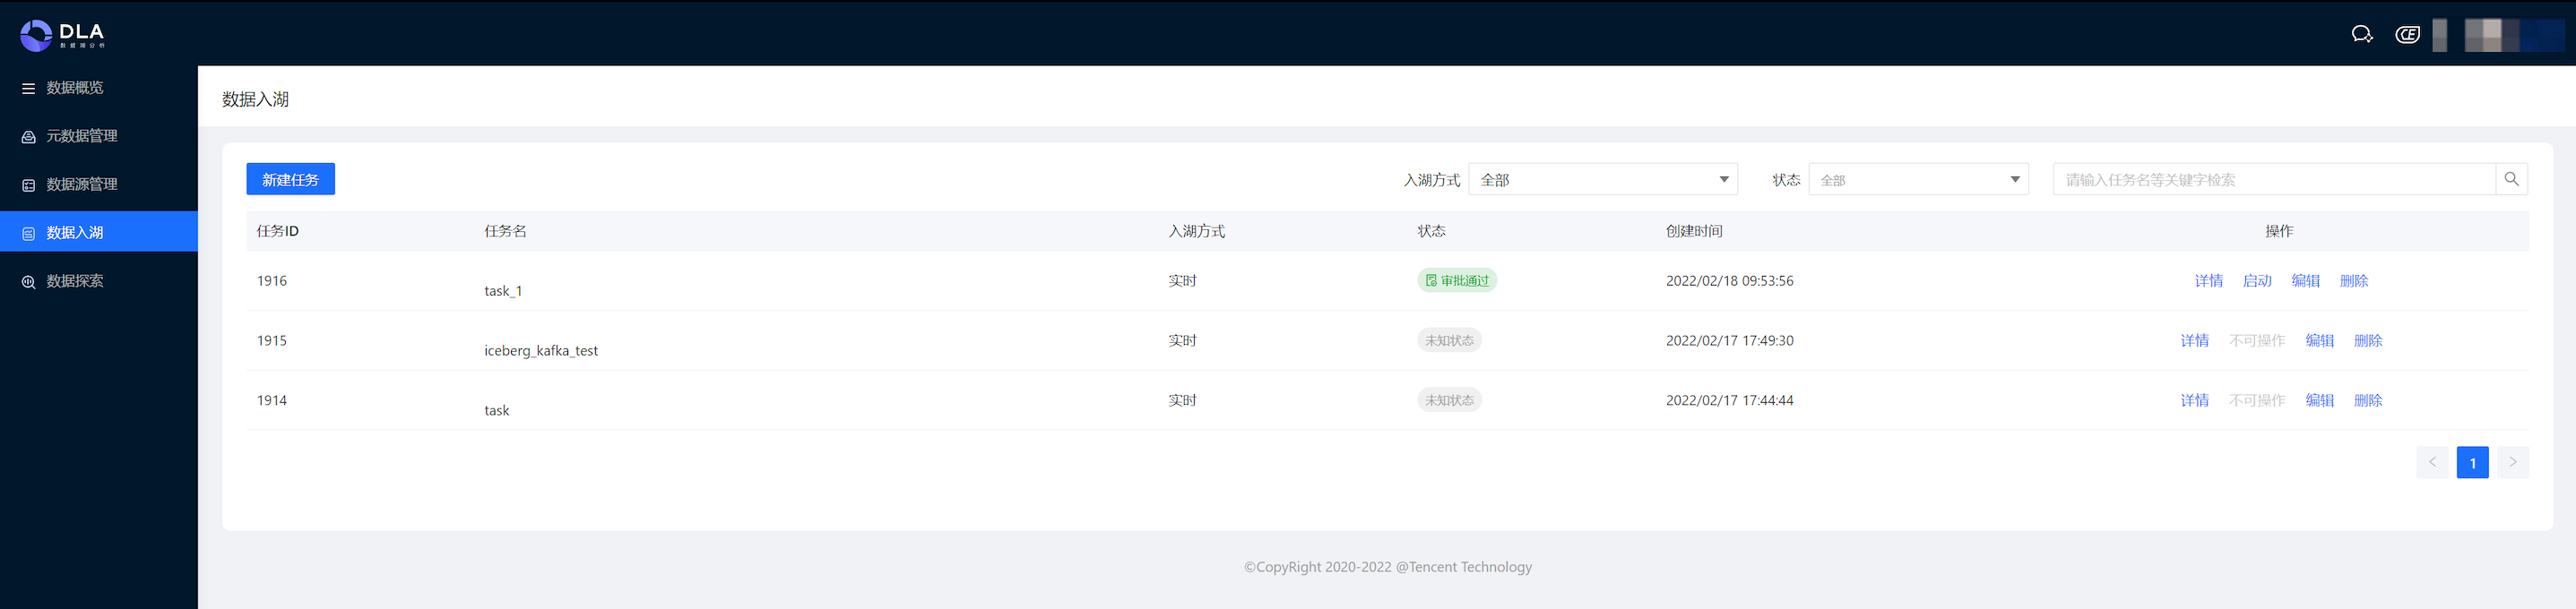
\includegraphics[width=1.0\textwidth]{数据入湖.png}
  \caption{数据入湖列表}
  \label{fig:数据入湖}
\end{figure}

相关的接口测试如下:

(1)创建实时任务接口测试如表\ref{tab:exampletable9}所示:

\begin{table}[H]
  \centering
  \caption{创建实时任务接口测试}
  \label{tab:exampletable9}
  \begin{tabular}{ll}
    \toprule
    接口描述         & 创建实时入湖任务         \\
    \midrule
    测试类型         & 功能测试         \\
    前置条件         & 后端服务器、 Hive Metastore、Oceanus平台正常         \\
    接口地址          & /formation/v1/tasks/streaming/createJob        \\
    请求方式         & POST      \\
    请求数据类型         & application/json     \\
    响应数据类型         & application/json,*/*           \\
    实际结果         & 达到预期结果           \\
    结论            & 测试通过           \\
    \bottomrule
  \end{tabular}
\end{table}

(2)创建存量入湖任务接口测试如表\ref{tab:exampletable10}所示:

\begin{table}[H]
  \centering
  \caption{创建存量入湖任务接口测试}
  \label{tab:exampletable10}
  \begin{tabular}{ll}
    \toprule
    接口描述         & 通过统一调度(US)创建存量表入湖任务         \\
    \midrule
    测试类型         & 功能测试         \\
    前置条件         & 后端服务器、Hive Metastore服务、US平台正常         \\
    接口地址         & /formation/v1/tasks/batch/createImportTask        \\
    请求方式         & POST      \\
    请求数据类型         & application/json     \\
    响应数据类型         & application/json,*/*           \\
    实际结果         & 达到预期结果           \\
    结论            & 测试通过           \\
    \bottomrule
  \end{tabular}
\end{table}

(3)获取任务列表接口测试如表\ref{tab:exampletable11}所示:

\begin{table}[H]
  \centering
  \caption{获取任务列表接口测试}
  \label{tab:exampletable11}
  \begin{tabular}{ll}
    \toprule
    接口描述         & 获取任务列表         \\
    \midrule
    测试类型         & 功能测试         \\
    前置条件         & 后端服务器、MySQL服务器正常         \\
    接口地址       & /formation/v1/tasks/getTaskList        \\
    请求方式         & GET      \\
    请求数据类型         & application/json     \\
    响应数据类型         & application/json,*/*           \\
    实际结果         & 达到预期结果           \\
    结论            & 测试通过           \\
    \bottomrule
  \end{tabular}
\end{table}

\subsection{数据探索}

在数据探索方面,Iceberg元数据存储在Hive Metastore中,因此可以通过统一查询平台进行数据查询和分析。
统一查询平台支持使用Presto和Spark进行数据探索,同时还提供了API接口,方便将数据输出到下游
的BI系统。除了统一查询平台,DLA还提供了Zeppelin来进行数据探索。Zeppelin的使用页面如图\ref{fig:Zeppelin使用}所示,
Zeppelin提供了用户友好的交互式界面
和支持多种编程语言的Notebook功能,用户可以通过编写SQL语句来进行数据查询和分析,并且可以将结果以多种
格式进行展示和分享。相关的测试可以直接在查询平台和Zeppelin上输入SQL语句进行测试。
总之,DLA为用户提供了多种数据探索工具和平台,方便用户进行数据的查询、分析和可视化。

\begin{figure}[H]
  \centering
  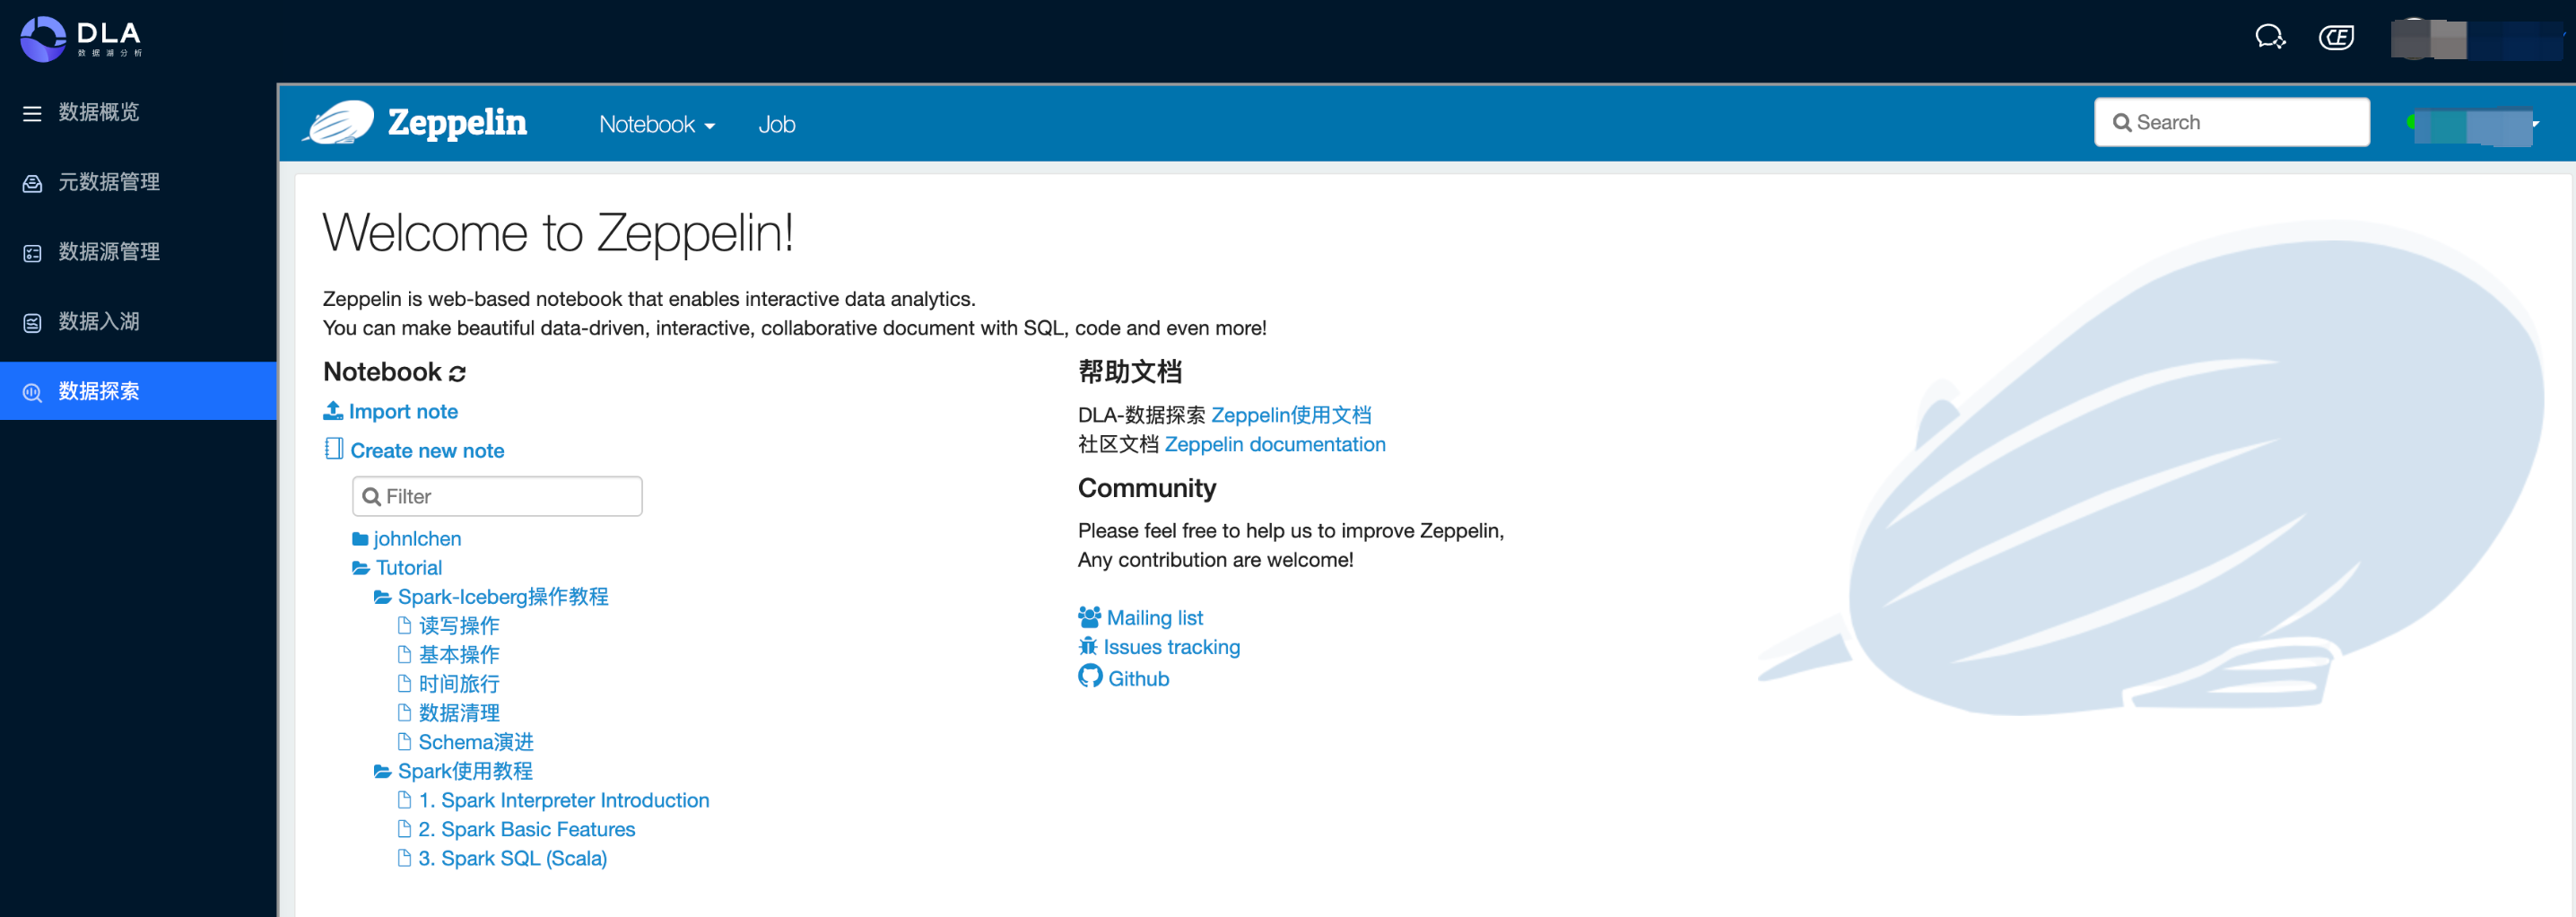
\includegraphics[width=1.0\textwidth]{Zeppelin使用.png}
  \caption{Zeppelin使用页面}
  \label{fig:Zeppelin使用}
\end{figure}

在统一查询平台上进行Iceberg表的查询如表\ref{tab:exampletable12}所示:

\begin{table}[H]
  \centering
  \caption{在查询平台上使用spark查询Iceberg表}
  \label{tab:exampletable12}
  \begin{tabular}{ll}
    \toprule
    测试描述         & 在查询平台上使用spark查询Iceberg表         \\
    \midrule
    测试类型         & 功能测试         \\
    前置条件         & Hive Metastore服务、查询平台正常         \\
    sql语句         & set supersql.execution.engine = spark;    \\
                   & select * from db.tbl1 a join db.tbl2 b on a.id = b.id limit 10;       \\
    实际结果         & 达到预期结果           \\
    结论            & 测试通过           \\
    \bottomrule
  \end{tabular}
\end{table}

使用Zeppelin进行查询的测试如图\ref{fig:badge1}所示:

\begin{figure}[H]
  \centering
  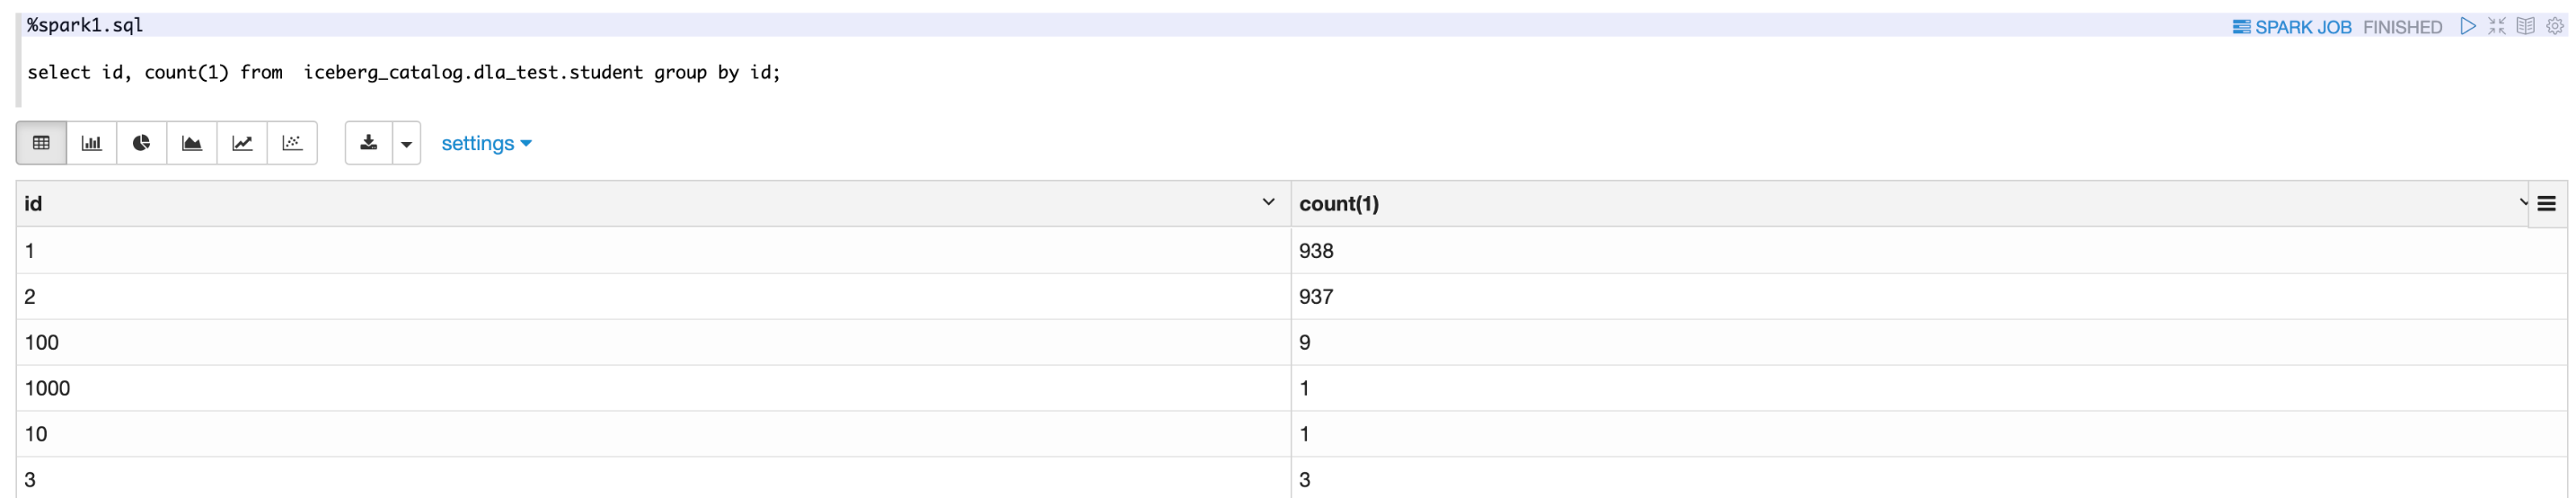
\includegraphics[width=1.0\textwidth]{zeppelin查询测试.png}
  \caption{Zeppelin查询测试}
  \label{fig:badge1}
\end{figure}

\subsection{自动优化服务}

自动优化服务是DLA为了帮助用户一键启动优化,摆脱之前运维成本高而设计的。用户可以在元数据页面看到
每个表都有一个优化的按钮,通过此按钮可以配置并启动Iceberg表的自动优化,当前支持的优化有小文件合并、
历史快照清除、孤儿文件清除、生命周期管理。配置数据优化服务和停止服务的测试如表\ref{tab:exampletable13}和\ref{tab:exampletable14}所示:

\begin{table}[H]
  \centering
  \caption{配置数据优化服务接口测试}
  \label{tab:exampletable13}
  \begin{tabular}{ll}
    \toprule
    接口描述         & 配置数据优化服务         \\
    \midrule
    测试类型         & 功能测试         \\
    前置条件         & 后端服务器、MySQL服务器、Hive Metastore、 \\
                   & US正常         \\
    接口地址       & /formation/v1/optimizer/configOptimizer        \\
    请求方式         & POST      \\
    请求数据类型         & application/json     \\
    响应数据类型         & application/json,*/*           \\
    实际结果         & 达到预期结果           \\
    结论            & 测试通过           \\
    \bottomrule
  \end{tabular}
\end{table}

\begin{table}[H]
  \centering
  \caption{停止数据优化服务接口测试}
  \label{tab:exampletable14}
  \begin{tabular}{ll}
    \toprule
    接口描述         & 停止数据优化服务         \\
    \midrule
    测试类型         & 功能测试         \\
    前置条件         & 后端服务器、MySQL服务器、Hive Metastore、 \\
                    & US正常         \\
    接口地址       & /formation/v1/optimizer/disableService        \\
    请求方式         & POST      \\
    请求数据类型         & application/json     \\
    响应数据类型         & application/json,*/*           \\
    实际结果         & 达到预期结果           \\
    结论            & 测试通过           \\
    \bottomrule
  \end{tabular}
\end{table}

对于数据优化的效果,进行了表\ref{tab:exampletable15}的测试:

\begin{table}[H]
  \centering
  \caption{数据优化效果测试}
  \label{tab:exampletable15}
  \begin{tabular}{ll}
    \toprule
    测试描述         & 数据优化效果测试,均在默认参数设置下         \\
    \midrule
    用户场景         & 2min一个checkpoint,一次checkpoint产生50个   \\
                   & 2MB的小文件,则一天会产生60 / 2 * 24 * 3=2000   \\
                   & 个元数据文件和60 / 2 * 24 * 50=36,000个2MB的     \\
                   & 小文件,按小时分区,数据保存30天,总大小2.16TB              \\
    不执行优化服务         & 元数据文件:2000 * 30 = 60000         \\
                        & 数据文件:36000 * 30=1080000个2MB的小文件         \\
    执行优化服务       & 元数据文件:约4700个(保留2天的快照文件 \\
                     & \hspace{2.2cm}和3天的metadata文件)        \\
                     & 数据文件:72000个2MB的小文件和 \\
                     & \hspace{1.85cm}21600个100MB的大文件        \\
    \bottomrule
  \end{tabular}
\end{table}

\section{系统非功能性性能测试}

系统非功能性测试主要进行了性能测试、端到端时延测试、安全性测试、可维护性测试和兼容性测试。
其中性能测试使用的是JMeter,JMeter是一个开源的性能测试工具,它可以用于测试Web应用程序、
Web服务、FTP、数据库、消息队列等各种应用程序的性能。JMeter支持多线程测试,
可以模拟大量用户同时访问应用程序,以评估应用程序的性能和稳定性。
JMeter还提供了各种图表和报告来帮助用户分析和解释测试结果。
JMeter具有简单易用的界面,用户可以通过图形化界面或脚本方式进行测试。

\subsection{性能测试}

本小节主要对数据湖分析系统的性能进行测试,以元数据管理为例,使用JMeter对系统的主要接口进行压力测试\cite{33},
测试用例如表\ref{tab:exampletable16}所示,测试结果如图\ref{fig:badge2}所示:

\begin{table}[H]
  \centering
  \caption{压力测试用例}
  \label{tab:exampletable16}
  \begin{tabular}{ll}
    \toprule
    测试描述         & 元数据管理性能测试         \\
    \midrule
    测试类型         & 性能测试         \\
    前置条件         & 用户成功登录系统         \\
    测试方法         & 使用JMeter模拟多用户进行压力测试        \\
    执行步骤         & 设置为1000个用户,每个用户访问10次,\\
                    &  在60s内完成      \\
    预期结果         & 总共10000个请求,平均响应时间在500ms  \\
                    & 内,百分之95的响应在1s内      \\
    实际结果         & 达到预期结果           \\
    结论            & 测试通过           \\
    \bottomrule
  \end{tabular}
\end{table}

\begin{figure}[H]
  \centering
  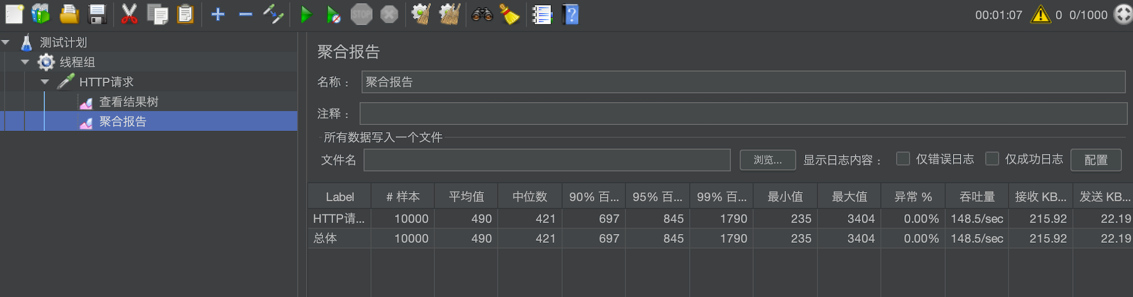
\includegraphics[width=1.0\textwidth]{压力测试结果.png}
  \caption{压力测试结果}
  \label{fig:badge2}
\end{figure}

\subsection{端到端时延测试}

端到端时延主要和数据导入延迟和数据查询延迟有关。对于数据导入延迟,将Kafka作为source进行了测试,
测试结果如表\ref{tab:数据导入}所示;对于数据查询延迟,使用presto进行查询时延测试,测试结果如表\ref{tab:数据查询}所示。

\begin{table}[H]
  \centering
  \caption{数据导入时延测试}
  \label{tab:数据导入}
  \begin{tabular}{ll}
    \toprule
    测试描述         & 数据导入时延测试         \\
    \midrule
    测试类型         & 时延测试         \\
    数据源           & kafka,每秒8W条record,每天大小1KB     \\
    任务资源         & flink集群提供20个CPU,每个CPU分配4G内存, \\
                   &  共80G内存     \\
    任务配置         & flink checkpoint时间设为1分钟,  \\
                    &  iceberg采用小时分区      \\
    预期结果         & 任务稳定运行,每个checkpoint都能按期完成  \\
    实际结果         & 达到预期结果           \\
    结论            & 测试通过           \\
    \bottomrule
  \end{tabular}
\end{table}

\begin{table}[H]
  \centering
  \caption{数据查询时延测试}
  \label{tab:数据查询}
  \begin{tabular}{ll}
    \toprule
    测试描述         & 数据查询时延测试         \\
    \midrule
    测试类型         & 时延测试         \\
    数据量          & iceberg表按小时分区,每个分区大约300G数据  \\
    sql语句         & set supersql.execution.engine = presto;    \\
                   & select * from db.tbl where partition = '2022120914' and id = xxx;       \\
    预期结果         & 1分钟内返回结果  \\
    实际结果         & 达到预期结果           \\
    结论            & 测试通过           \\
    \bottomrule
  \end{tabular}
\end{table}

\subsection{安全性测试}

系统安全性测试是一种重要的测试方法,可以评估系统在安全方面的弱点和漏洞,并发现和修复潜在的安全问题。
数据湖分析系统的安全性主要是借助内部的安全中心实现的,用户通过安全中心的权限认证后,才能进行相关元数据的操作以及
资源的申请,测试用例及其结论如表\ref{tab:安全性测试用例}所示:

\begin{table}[H]
  \centering
  \caption{安全性测试用例}
  \label{tab:安全性测试用例}
  \begin{tabular}{ll}
    \toprule
    测试描述         & 系统安全性测试         \\
    \midrule
    测试类型         & 安全性测试         \\
    前置条件         & 用户在安全中心没有创建iceberg的权限       \\
    执行步骤         & 用户在元数据管理页面进行表的创建\\
    预期结果         & 创建失败  \\
    实际结果         & 达到预期结果           \\
    结论            & 测试通过           \\
    \bottomrule
  \end{tabular}
\end{table}

\subsection{可维护性测试}

在系统维护方面,建立了相应的流水线来进行升级和回滚,在升级流水线中,还对
代码复杂度、代码重复度、代码可读性、代码注释、代码测试覆盖率等进行了评估,以帮助开发团队识别和改进软件系统的潜在问题。
对流水线进行的测试如表\ref{tab:可维护性测试用例}所示:

\begin{table}[H]
  \centering
  \caption{可维护性测试用例}
  \label{tab:可维护性测试用例}
  \begin{tabular}{ll}
    \toprule
    测试描述         & 可维护性测试用例         \\
    \midrule
    测试类型         & 升级流水线测试         \\
    前置条件         & 升级流水线成功构建       \\
    执行步骤         & 在代码仓库中发布新的版本\\
    预期结果         & 升级成功  \\
    实际结果         & 达到预期结果           \\
    结论            & 测试通过           \\
    \bottomrule
  \end{tabular}
\end{table}

\subsection{兼容性测试}

系统兼容性测试旨在评估软件系统在不同硬件、操作系统、浏览器、移动设备等不同环境下的兼容性。
以帮助开发团队发现和解决软件系统在不同环境下的兼容性问题,以确保软件系统能够在各种环境下正常运行和提供一致的用户体验。
这里仅对不同的浏览器进行测试,相关的测试用例如表\ref{tab:兼容性测试用例}所示:

\begin{table}[H]
  \centering
  \caption{兼容性测试用例}
  \label{tab:兼容性测试用例}
  \begin{tabular}{ll}
    \toprule
    测试描述         & 兼容性测试用例         \\
    \midrule
    测试类型         & 兼容性测试         \\
    前置条件         & DLA前端和后端正常运行   \\
    执行步骤         & 分别在Google、Firefox、360浏览器、  \\
                   & Safari浏览器上进行DLA的体验   \\
    预期结果         & 在各浏览器上均能正常使用  \\
    实际结果         & 达到预期结果           \\
    结论            & 测试通过           \\
    \bottomrule
  \end{tabular}
\end{table}

\section{本章小结}

本章主要介绍了系统功能性测试和非功能性测试。在系统功能测试中对系统各个
功能模块设计了大量的接口测试,并且根据测试结果对系统设计方案进行了改进,
本章只列举了部分关键接口测试。在系统非功能性测试中主要进行了性能测试、端到端时延测试、安全性测试、可维护性测试和兼容性测试,
测试结果符合预期。
